% Chapter 4 from the standard thesis template
% that contains an adv. example table and figure.
\chapter{SOFTWARE DEFINED RADIOMETER IMPLEMENTATION}\label{ch:implementation}

\section{Introduction}
One of the principal goals with this research was to implement a fully functioning total power radiometer within software.  The N200 provides us the link between the RF signal captured by the antenna and converts that to a format that can now be used by the to manipulate the signal.  Once the signal has been passed to the computer, GNURadio will implement the correct algorithms to detect the power within the signal, filter and output the information.  One of the advantages of course with a SDR is that filtering can also be done within the software.  In addition, thanks to the WxGUI that GNURadio uses, we can also build a user interface that can control several key variables that are useful for us.  This includes controlling the gain on the programmable gain amplifier on the DBSRX2 card, the sampling or bandwidth of the signal, the center frequency, and also the integration time.  All of these can now be controlled in real time as well.  GNURadio will also store the power data so that we are able to do further analysis of the data using a software program like Matlab or Python.  Because GNURadio is a very flexible system we are able to do more with the signal such as filtering, polarimetric  radiometer, and frequency analysis.  We are also able to add additional features and improvements through updates to the software.

\section{Requirements}

To help us quantify the required performance of the radiometer, we referred to information provided to us by Dr. Brian Hornbuckle but also derived from existing radiometers.  As stated earlier, although a radiometer measures power, we often convert this to an equivalent brightness temperature.  Specifically, we are looking at the brightness temperature of the antenna added to the brightness temperature of the object of interest.  We also have to be able to detect a minimum amount of power.  Since changes in noise can be small, the better the sensitivity of the radiometer, the better we can detect these small changes.  

The requirements given are outlined in the table below.

\begin{table}[h!tb] \centering
\isucaption{Required Radiometer performance}
\label{rad_performance}
% Use: \begin{tabular{|lcc|} to put table in a box
\begin{tabular}{lcc} \hline
\textbf{Parameter} & \textbf{Value} & \textbf{Units} \\ \hline
Minimum bandwidth & 20 & MHz \\
Operational frequency & 1400 - 1420 & MHz \\
$NE\Delta T$ & 1 & Kelvin \\ \hline
\end{tabular}
\end{table}



%----------------------------------------------------------
% End of Chapter 4.  Anything below this is extra information


\section{Square-law Detector Performance}
The Square-law detector was added to our system in order to give us another reference point and to help verify the power output that the software defined radio.  Performance of our square-law detector is based on two items; the sensitivity of the diode used in the square-law detector and the analog to digital converter used to convert the analog voltage to a digital value.  The sensitivity of this device accounts for most of the performance factor of the system.  In our system the output of this square-law detector is then feed directly into an analog to digital converter.  Therefore, the performance of this A/D converter needs to be accounted for as well [\cite{Terlep}].  

For our square-law detector, it has a noise output of $25nV/ \sqrt{Hz}$ at 100 kHz and will detect a signal as low as $-60$ dBm.  This works will with our needs since the RF front end brings the noise floor to approximately $-30$ dBm.


\section{Software Defined Radio Performance}
Performance of the software defined radio is governed by the system that takes in the RF signal and then digitizes the signal.  Once the signal is in digital form, we no longer are concerned about loss of performance due to additional noise that may get added to the system.  For this reason, we attempt to digitize the signal as soon as possible.

For the N200 this is done by the DBSRX2 daughter-board that plugs into the N200 base system.  While this board does play a part in the overall system performance, because this sits later in the chain however the impact to the performance is low as shown in equation \ref{noise_factor}.  However, this module does need to be in the frequency range of the radiometer, or in our case 1.4 GHz.  This board meets that criteria.  Ideally, we still want the noise figure on this board as low as possible, even though the impact is low.  The DBSRX2 does meet this having a noise figure of approximately 5 dBm.


Requirements for this system was based on information provided by Dr. Brian Hornbuckle and was also based on requirements of a typical radiometer.  This list is outlined in table~\ref{requirements} shown below.

\begin{table}[h!tb] \centering
\isucaption{ISU Radiometer requirements}
\label{requirements}
\begin{tabular}{lcc} \hline
\textbf{Requirement} & \textbf{Value} & \textbf{Units} \\ \hline
Frequency Range & 1400 - 1420 & MHz \\
Bandwidth & 20 & MHz \\
Polarization & Dual &  \\ 
Sensitivity & -30 & dBm \\
Accuracy & 1 & Kelvin \\ \hline
\end{tabular}
%\vspace{ 2 in}
\end{table}

\subsection{Hardware Requirements}

The selection of the N200 SDR from Ettus Research was based on many of the requirements outlined in table~\ref{requirements}.  In addition, we wanted the hardware to be flexible but also affordable.  There are many kinds of software defined radios on the market.  However, we choose the N200 based on the availability of the device, the large community support, especially with regards to support by GNURadio, and because it meets and often exceeded the requirements stated above.  

Flexibility was another key aspect of the N200 that made it an excellent selection for this research.  The N200 uses a daughter board setup for bridging the RF interface to the rest of the electronics.  Several daughter boards are available that have different frequency ranges and offer both receive, transmit and transceiver designs.  For the radiometer we need to operate around 1.4 GHz and receive only.  Based on those requirements we choose the DBSRX2 daughter board.  This board is designed from 800 MHz to 2.3 GHz and has a fairly low noise figure.

The current RF front end to the radiometer is designed for a 20 MHz wide signal.  This requirement was one of the main driving points for selecting the N200 SDR as it can support up to 50 MHz in bandwidth between the N200 and the host computer.  This is accomplished by using a 1 Gbps Ethernet connection between the N200 and the host computer.

\subsection{Software Requirements}

The driving force for the software requirement was to have a system that was easy to use yet powerful enough to handle the amount of data that is required.  One reason for the development of this platform is to make radiometers more accessible to other researchers and other programs such as education and even amateur radiometer work.  Therefore, ease of use was taken into consideration when selecting the hardware and the associated software used with it.

The data flow model for the hardware selected uses the FPGA to perform low level signal processing on the signal and moves high level processing to the host computer.  This allows for less processing requirements on the physical hardware but requires a host computer that is able to process the incoming information.  It also requires a software package that is able to process this information efficiently. 

Because a requirement is an easy to use system GNURadio was selected as it includes GNURadio Companion (GRC). GRC is a supplemental program which uses a graphical interface for creating the radio environment.  It also includes options to create a user interface during the operation of the N200 as well.  This allowed us to rapidly create both the critical radio components needed for the radiometer and also a control interface.

This software meet the criteria of allowing a simple to use interface to be built and used in the control and data recording of the information required.  It also uses a simple interface for making changes to the program.  These changes can be both in the GUI and also to how the program processes the information.

\section{Software Defined Radiometer Theory of Operation}

\section{Mapping analog radiometer functions to a software defined radiometer}

In order to recreate a radiometer in software we need to identify the key components of a radiometer and then recreate those components in software.  As discussed in chapter three, the three components identified that are key to a radiometer is listed below.

\begin{enumerate}
\item Power detection
\item Integration
\item Bandwidth limitation or filtering
\end{enumerate}

The following sections will now examine how these items are mapped from their analog component to the software or digital component.
\subsection{Power detection}
Power detection is a key ability that allows a radiometer to function.  At its core a radiometer is a power detector.  Therefore, the implementation of power detection is a crucial function of a software defined radio radiometer.

To implement a total power radiometer in software we first need to look at how we implement a total power radiometer traditionally.  Traditionally, a square law detector is used to detect the average power that is seen by the radiometer.  This simple device uses a diode that gives a small voltage output based on the RF power present.  This small voltage is then amplified and can now be calibrated with a known source to give us a noise temperature.  

{\begin{figure}[h!tb] 
\centering
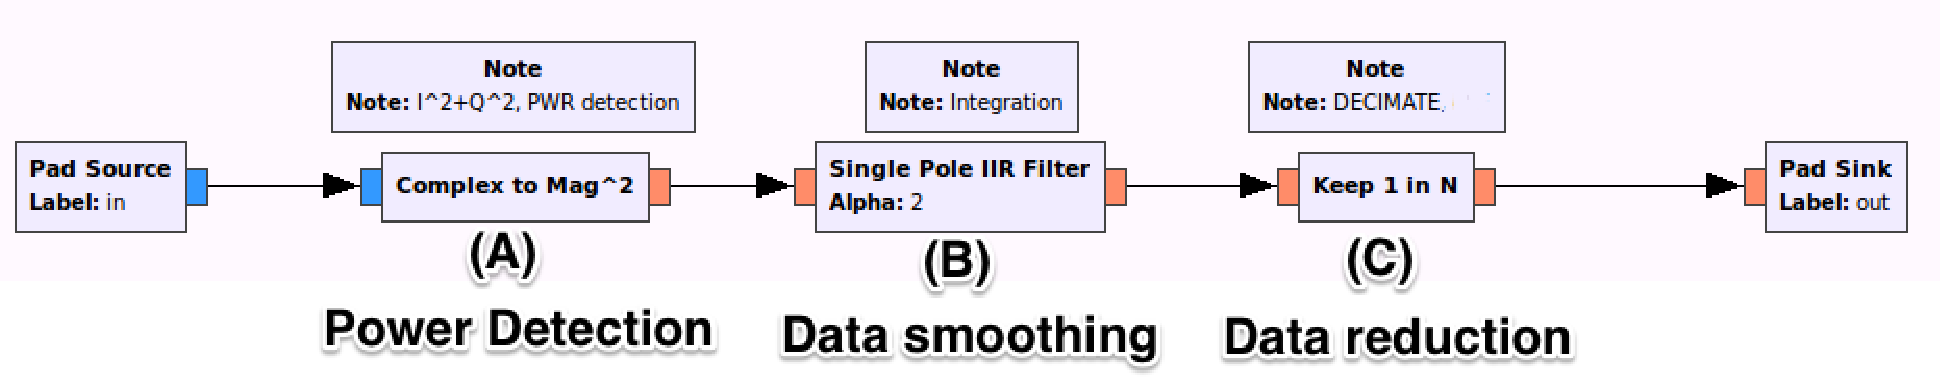
\includegraphics[width=17cm]{Images/TPR_grc.png}
\isucaption{A block diagram showing how the radiometer performs the equivalent square law detector in software.}
\label{square_block}
\end{figure}
}

To implement this in software we need to build a square law detector mathematically.  We can then give this to the software defined radio to process the information accordingly.  A square law detector mathematically is the sum of the squares.  Once the signal has been digitized, it is expressed in data bits of I and Q, which represent in-phase and quadrature-phase of the signal.  By squaring each term, we get the desired result of the power of the signal [\cite{Sarijari}][\cite{Rashid}] can be shown in equation \ref{sdr_x2}.

\section{Integrator through a IIR Filter}

Another step that we typically do in a traditional radiometer is to integrate the signal over time.  This gives us an average of the signal and smooths out the output.  In addition, we will show later that the integration time can be adjusted to help improve our sensitivity of the radiometer.

In a traditional radiometer, we can integrate by using a simple integrator circuit, which consists of an op-amp, resistor and capacitor.  This circuit configuration is also equivalent to a low pass filter circuit as well, and the two are interchangeable.  We can then look at how we filter in the digital domain, and this is down with an infinite impulse response filter or IIR.  We can use this digital filter to then integrate the signal for our total power radiometer. Again, this relationship between the IIR filter and the integrator is explained in chapter 2 and is mathematically shown in equation \ref{final_IIR_RC}.


\subsection{Software Defined Radio Radiometer}

A Software defined radio consist of both hardware and software that allow it to perform the operations of a radio or communication channel.  A software defined radio used for radiometer applications is identical to a software defined radio used for, as an example, a 802.11b radio with one major difference.  Since we need to amplify the signal more than what most communication applications require; we do require more powerful or additional LNAs to boost this signal.  In addition, since the first LNA plays a major role in the overall system noise and this system noise does affect performance of the radiometer, the selection of this LNA is important.  However, all other components are the same components used in other applications.

A software defined radio radiometer behaves analogous to a more traditional radiometer and thus the application is the same as a traditional radiometer.  This includes applications such as radio astronomy that includes applications in Earth Science such as soil moisture and ocean salinity[\cite{Ruf}].  A software defined radio radiometer can also allow for new application development that can expand the remote sensing field.  Since we have moved the majority of the hardware to software this allows us to further shrink the size and weight of the radiometer.  This allows for other radiometer applications such as Unmanned Aerial Vehicles (UAVs) for scanning soil moisture and ocean salinity remotely[\cite{McIntyre}].  

We will now introduce the three major components that make up a software defined radio radiometer.  

%\textbf{N200 SDR}
\subsubsection{N200 Software Defined Radio} 
The key component for a software defined radio radiometer is the software defined radio or SDR that will do most of the work as a radiometer through software.  The equipment selected for researching into this topic was the Ettus Research Group N200 SDR.  The SDR selected utilizes daughter boards as the RF front end to the SDR and up to two daughter boards may be installed into a N200.  This is an important consideration as one of the requirements is to be able to look at both the V-Pol and the H-Pol signal coming from the antenna.  By having a dual receiver SDR it is possible to correlate the signal and other signal analysis can also be done.  Another important reason the N200 is selected was due to its ability to handle up to 50 MHz of bandwidth to the computer and up to 25 MHz of RF bandwidth per daughter-board plugged in to the SDR.  This means that it is possible to have two receive cards that can stream up to 25 MHz bandwidth each.  

The N200 utilizes a flexible architecture for a variety of RF interface systems based on the frequency range desired and if receive and/or transmission is needed.  These daughter boards directly receive the RF signal and then outputs the analog I and Q signals that are then sampled by the N200 A/D converter for reception or receives the I and Q values from the N200 D/A converter for transmission. 

{\begin{figure}[h!tb] 
\centering
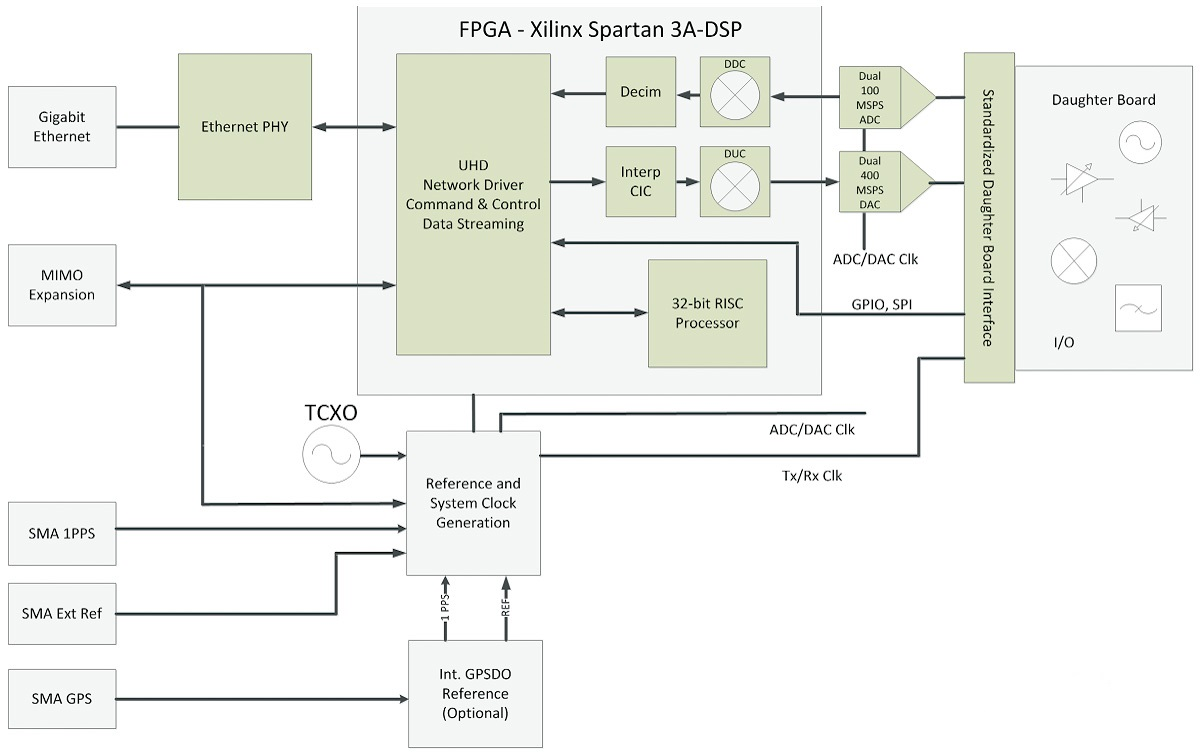
\includegraphics[width=14cm]{Images/n200_block_edited}
\isucaption{A block diagram of the Ettus N200 SDR}
\label{N200_block}
\end{figure}
}

The daughter board selected is the DBSRX2 card as this card is receive only and operates between 800 MHz and 2.4 GHz.  The DBSRX2 also has built in amplification that is adjustable through software.

\subsubsection{GNURadio Software}

For the software portion of the radio, we settled to use GNURadio, an open source software package that is well supported by the community and by the Ettus Research Group and the N200 SDR.  GNURadio also comes with what is known as GNURadio Companion or GRC.  This program provides us with a GUI interface and allows for the drag and drop of blocks that represent certain functions that can be used with the SDR.  GNURadio and GRC use Python as its main scripting language and GNURadio uses C++ code for directly accessing the hardware.  The hardware interface for the N200 is provided by Ettus through drivers that allow GNURadio to talk to the hardware.  Like GNURadio, these drivers are also available to all platforms.  Ettus has released these drivers to the open source community and continues to support the hardware drivers and GNURadio integration.

GNURadio operates on multiple platforms including Windows, Mac OS X, and Linux.  Linux is by far the most popular platform to work on and most of this thesis research was completed within the Linux environment.  Testing is also done though with a MacBook Pro running OS X 10.9.  The OS X implementation is well supported and is installed through MacPorts.  While windows is technically supported, it is often difficult to install and many of the libraries required are not 64-bit.  For these reasons windows was not used for executing GNURadio, but was used for some of the data analysis using Python.

Through GNURadio, we can now write code that will take the data given to us from the SDR and manipulate the signal as we need to mimic a radiometer.  The power detection, filtering and recording of this data is all done through GNURadio.  This also means that we are shifting more of the computational power done on the signal from the FPGA to a computer running GNURadio.  There are ways to change this behavior and upload code directly to the FPGA.  However, for this thesis it was easier to debug and work with GNURadio by keeping the processing on the desktop computer.  It does however mean that the host computer must be powerful enough to handle the signal and specifically the large bandwidth that we wish to send to it.  

\subsection{RF Front End}
The RF front end plays a critical role in the radiometer as the LNAs used in the front end has a large impact on the system noise generated by the radiometer itself.  A traditional radiometer utilizes both amplification through the LNAs and also includes filtering to the desired bandwidth.  A SDR radiometer does not require the filters as we are able to create these in software, however the amplification stages need to remain.  

{\begin{figure}[h!tb] 
\centering
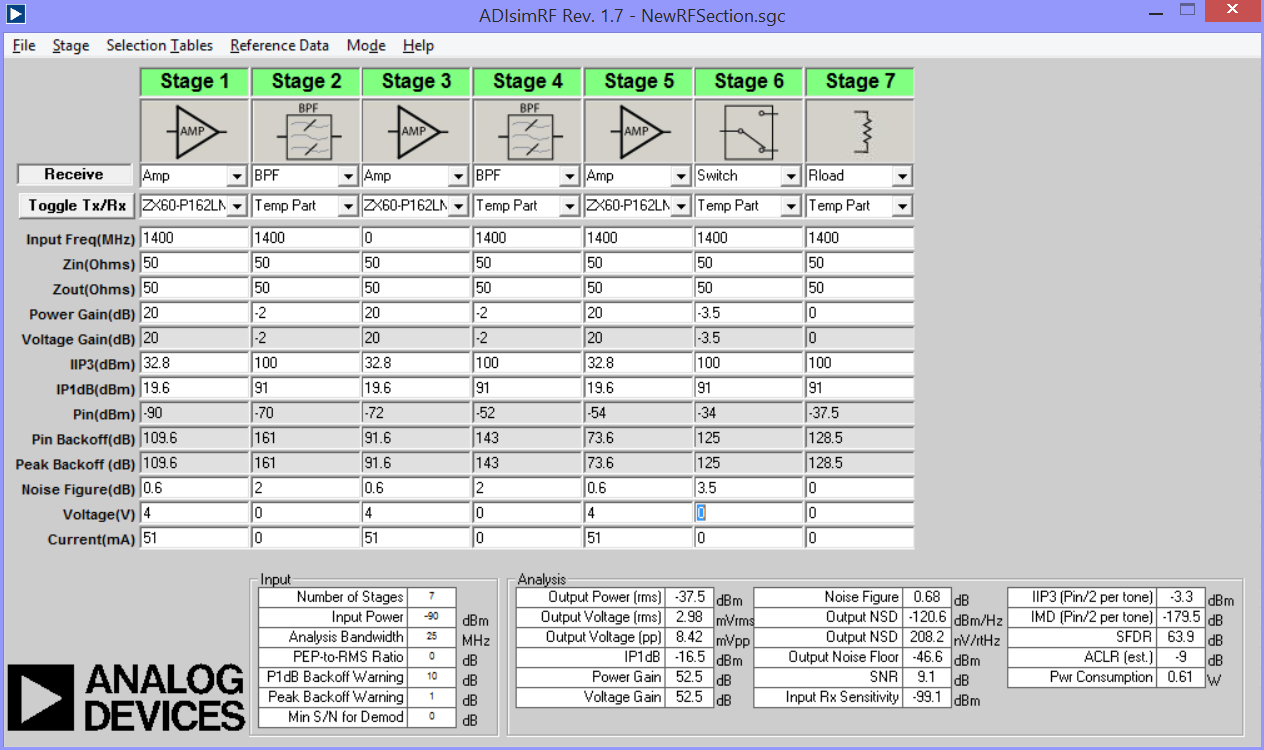
\includegraphics[width=0.8\linewidth]{Images/RF_Front_end.png}
\isucaption{The ADISIMRF program used to verify the design of the RF Front End}
\label{ISU_Rad}
\end{figure}
}
A typical RF front end uses a 3 stage Low Noise Amplifier (LNA) to amplifier the noise while keeping the noise contributed to the system as low as possible.  As with any radiometer, the first LNA is the most critical as it contributes the most to the overall system noise temperature.  For this reason a LNA that did not have a large gain but had a low noise figure is chosen. The second and third LNA has higher gain values at the cost of a higher noise figure, although not by much.  However, since they are further down the chain, they do not contribute as much to the total system noise.  The reason for this is further explained in chapter 3. 


\subsection{Software Defined Power Detection}

A traditional radiometer uses a square-law detector which takes the input signal and produces a voltage that is proportional to the square of the voltage.  This allows us to take an analog RF signal and convert the noise voltage that for all intense and purposes has a mean value of zero, and produce a noise power.

For a SDR, the incoming signal is sampled and converted to I/Q values by the hardware within the SDR.  The I/Q values together can be used to reconstruct both the phase, frequency and amplitude information of the signal and can do so much more accurately then if we just recorded the frequency and amplitude information.  In GNURadio we are then able to square these values within software which give us our peak voltage of the signal.  This block in GNURadio mathematically performs what is shown in equation \ref{sdr_x2}.

\begin{equation}\label{sdr_x2}
I^2+Q^2 = P_{out}
\end{equation}

Therefore, like the analog square-law detector we are taking peak voltage values, which has an equivalent noise voltage and a mean value of zero, and square them to produce a noise power that is proportional to the square of this amplitude.

Like the analog square-law detector, this signal will fluctuate rapidly and to improve the sensitivity of the radiometer we wish to integrate this signal.  We now want to look at how we can replicate a RC filter or integrator in the software defined radio.

\subsection{Software Defined Integrator}
A RC filter is analogous to an integrator where the R and C values determine our time constant and our integration time for the filter[\cite{Aitken}].  We know a RC filter is analogous to an integrator by looking at equation \ref{eq:rc_int}.  A SDR however operates in the digital domain at discrete intervals.  One type of filter that can be used is the Infinite Impulse Response (IIR) filter. 

\begin{equation}\label{eq:rc_int}
\frac{1}{RC}\int{V_idt}
\end{equation}


To begin with, we look at what an analog RC filter looks like. 

{\begin{figure}[h!tb] 
\centering
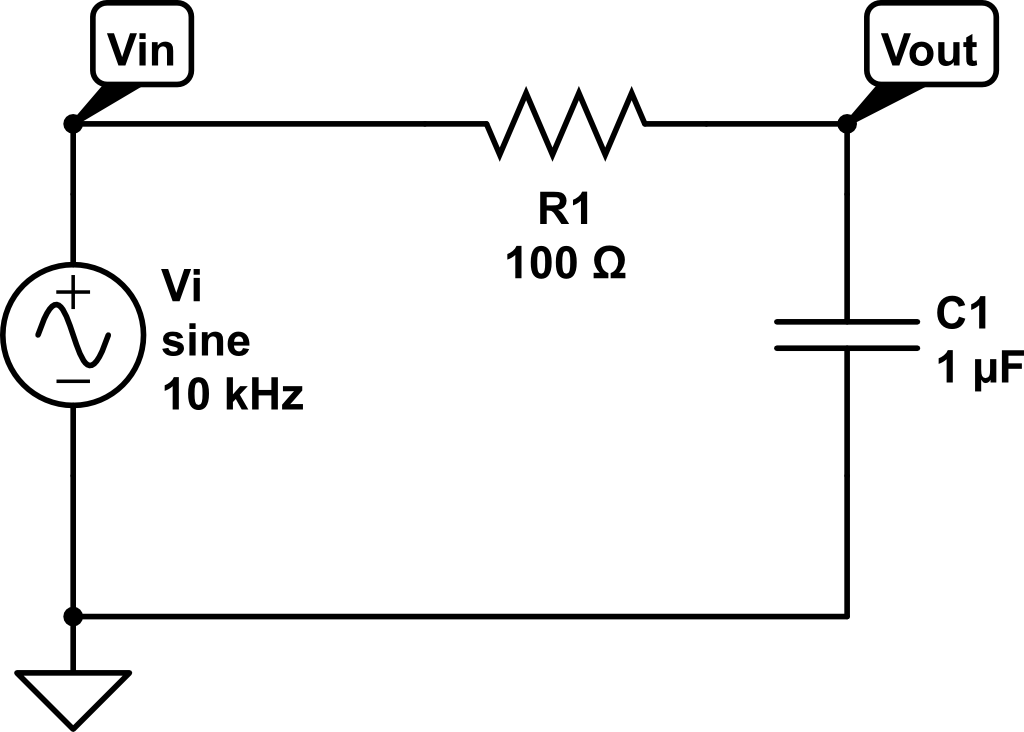
\includegraphics[width=10cm]{Images/rc-circuit.png}
\isucaption{A simple RC circuit}
\label{rc_circuit}
\end{figure}
}

This circuit can be represented by equation \ref{eq:rc_circuit_eq}.

\begin{equation}\label{eq:rc_circuit_eq}
\frac{V_{in}-V_{out}}{R}=C\frac{dV_{out}}{dt}
\end{equation}

A Finite Impulse Response (FIR) filter is a digital filter that can take an impulse signal and decays to zero after a finite number of iterations.  This type of digital filter can be represented by equation \ref{FIR_Eq} which mathematically expresses the FIR Filter.

\begin{equation}\label{FIR_Eq}
y_n=\displaystyle\sum\limits_{i=o}^{P-1} c_ix_{n-i}
\end{equation}

This simply says that the nth output is a weighted average of the most recent P inputs.  

An Infinite Impulse Response (IIR) filter is the same as the FIR filter, except that we add a summation term which feeds back the previous output.

\begin{equation}\label{IIR_eq}
y_n=\displaystyle\sum\limits_{i=o}^{P-1} c_ix_{n-i}+\displaystyle\sum\limits_{j=1}^{Q} d_jy_{n-j}
\end{equation}

Equation \ref{IIR_eq} shows that a FIR filter is a IIR filter, except that $Q=0$[\cite{Cross}].  

To get a better understanding on how the digital IIR filter relates to the RC filter analog, we can look at the Fourier Transform and the relationship of the input to the output in the frequency domain.

\begin{equation}\label{Fourier_IIR}
H(f)=\frac{\displaystyle\sum\limits_{j=o}^{P-1} c_je^{-2\pi ijfT}}{1-\displaystyle\sum\limits_{k=1}^{Q} d_ke^{-2\pi ikfT}}
\end{equation}

In equation \ref{Fourier_IIR}, $f$ is our frequency in Hz and $T$ is the time between samples in seconds and is related to our sampling frequency.

We now want to show the link between our analog RC circuit and the IIR filter.  Looking at equation \ref{eq:rc_circuit_eq}, which represents the differential equation relating the input voltage $V_{in}$ to the output voltage $V_{out}$, we can substitute for input and output of our IIR filter.  Since we are now in the time domain, we need to define what $T$ is and we can do that using equation \ref{sampling_rate_eq}.

\begin{equation}\label{sampling_rate_eq}
T=time between samples=\frac{1}{sampling rate}
\end{equation}

We can now relate our input voltage to the input to our IIR filter and the output voltage to the output of our IIR filter.

\begin{equation}\label{input_IIR}
x_n=v_{in}(nT)
\end{equation}

\begin{equation}\label{output_IIR}
y_n=v_{out}(nT)
\end{equation}

We can now rewrite our difference equation with $x_n$ and $y_n$.

\begin{equation}\label{diff_xn_yn}
\frac{x_n-y_n}{R}=C\frac{y_n-y_{n-1}}{T}
\end{equation}

Finally, we can solve for $y_n$ which results in our final equation for showing how a IIR filter is related to an RC filter.

\begin{equation}\label{final_IIR_RC}
y_n=\frac{T}{T+RC}x_n+\frac{RC}{T+RC}y_{n-1}
\end{equation}

It can be seen that an IIR filter can have the same frequency response as we expect from an analog RC filter.  As our sampling rate approaches infinity, the approximation gets closer to the original response from the analog RC circuit.  

For the cutoff frequency of a RC circuit, we know that it has the relationship shown in equation \ref{RC_relationship}.

\begin{equation}\label{RC_relationship}
f_c=\frac{\sqrt{3}}{2\pi RC}\rightarrow RC=\frac{\sqrt{3}}{2\pi f_c}
\end{equation}

The $RC$ term gives us our time constant of the circuit and can be used to calculate out our coefficients.  We are not concerned about the actual values of R and C with our IIR filter, instead we just need the product of R and C.  

In GNURadio most of the work is done for us.  We can simply enter in our desired cutoff frequency and GNURadio will calculate our IIR filter coefficients.  However, this shows that an IIR filter works much like an analog RC low pass filter.

Like a traditional radiometer, the SDR will use an antenna to look at the target of interest.  SDRs still use a RF stage that takes the power from the source and amplifies it.  The difference though begins after that.  A SDR will then sample and generate I and Q values that represents the amplitude and phase of the signal.  From there, this data is sent to a computer to be processed.  We can then use this information to calculate the power that is being seen.  In addition, we can manipulate the signal in other ways such as applying a filter to filter out an unwanted source.

\subsection{SDR Radiometer Summary}

As we have shown the two of the major components of a traditional radiometer, the power detection and integration of the signal can be replicated in software and therefore can be implemented in a software defined radio.  The information can now be stored, displayed or both for further analysis.  

There is one component of the software defined radio that we are not able to implement in software and that is with the signal amplification.  This however does play a major role in the performance of the radiometer and is a key element that should not be overlooked.  While this is not implemented in software, it still plays a critical role in our software defined radio radiometer. 

\subsection{RF Front End}

Hardware with a software defined radio still plays a critical role.  A traditional software defined radio will focus on digitizing the signal as soon as possible and the hardware used will be focused on performing that critical digitizing process.  For a software defined radio radiometer, we still want to digitize as soon as possible, but we also need to consider our noise factor.  Most software defined radios are designed for communication purposes such as implementing 802.11b or other wireless protocols.  In these scenarios a higher noise factor is not as detrimental to the overall system as it is with a radiometer.  This is because we have a known signal that is magnitudes greater than the noise floor.  In a radiometer however, we do not have this large separation between the information we need and the noise of the system.  And so our noise factor is a more critical component.  

To counter this, we use Low Noise Amplifiers to amplify the signal but it can also help lower our noise factor.  The first LNA in the chain contributes a large amount to our noise factor, so by selecting a LNA that has a low noise factor, it reduces the noise factor for the system.  This can be shown by looking at the equation that calculates our noise factor.

\begin{equation}\label{noise_factor}
F=F_1+\frac{F_2-1}{G_1}+\frac{F_3-1}{G_1 G_2}+\frac{F_4-1}{G_1 G_2 G_3}+\cdots +\frac{F_n-1}{G_1 G_2 G_3 \cdots G_{n-1}}
\end{equation}

While additional components do add to the noise figure, their contribution is significantly lower than the first LNA put in the RF chain.

This however is the only major change we need to do for doing radiometer work with an off the shelf radiometer.  The rest will be done within software which is the principal reason for using a software defined radio.

\section{General Specifications}
In general, since we are digitizing the signal early in the RF signal chain, the noise figure of the RF components in the SDR do not add a significant amount of noise to the system.  Additional performance metrics that require examination include how much bandwidth the system can handle.   The information below outlines the specification of the devices used and its impact on the performance of the SDR as a digital radiometer.   

\section{Comparison of a Software Defined Radio Radiometer vs Traditional Radiometer}

As outlined above, a software defined radio implements a traditional radiometer but in the digital domain.  For power detection, we simply sum the squares of the I and Q values that have been sampled by the software defined radios analog to digital converters.  As with a traditional radiometer, we also want to filter this information to remove much of the jitters that comes from the rapid fluctuations in the power readings.  This is done using an IIR low pass filter, which mimics a traditional RC low pass filter.  Once completed, we now have the total power reading from the radiometer and we can now store, display or do both with this information.  

A traditional radiometer may also use an analog to digital converter in order to digitize the analog voltage from the square-law detector.  Because the sample rate of this voltage is low, almost any analog to digital can be used for this.  At this point however, there is no frequency information, only the magnitude information is being retained and recorded.

%----------------------------------------------------------
% End of Chapter 4.  Anything below this is extra information
